\documentclass[11pt, oneside]{article}
\usepackage{lmodern} % Use scalable fonts to avoid font substitution warnings
\usepackage{tikz-cd} % Commuting diagrams
\usepackage[a4paper, margin=1in]{geometry} % Adjust margins
\usepackage[noxy, goodsyntax]{virginialake} % Typesetting derivations
\usepackage{xcolor}
\usepackage{amsthm} % Theorem environments
\usepackage{titlesec}
\usepackage{amsmath} % Symbols
\usepackage{graphicx} % Better figures
\usepackage{caption} % Figure captions
\usepackage{mathtools} % '\denote' command
\usepackage{stmaryrd} % Double brackets
\usepackage{cancel} % Negataing coherence relations
\usepackage{bm} % Bold maths expressions
\usepackage{changepage} % Indenting sections in proofs
\usepackage{tocloft}
\usepackage{tikz} % Structure bracket heirarchy

\usetikzlibrary{arrows.meta, positioning}
\setlength{\cftbeforesecskip}{11pt}  % Adjusts spacing before section entries
% Remove paragraph indentation
\setlength{\parindent}{0pt}
% Add space between paragraphs
\setlength{\parskip}{1em}

\titleformat{\section}[block]{\normalfont\bfseries\fontsize{1.3em}{1.3em}\selectfont}{\thesection}{1em}{}

\theoremstyle{plain}
\newtheorem{theorem}{Theorem}[section] 
\newtheorem{proposition}[theorem]{Proposition}
\newtheorem{lemma}[theorem]{Lemma} 
\theoremstyle{definition}
\newtheorem{definition}[theorem]{Definition}
\newtheorem*{remark}{Remark}
\newtheorem{example}[theorem]{Example}
\usepackage{etoolbox}
\AtBeginEnvironment{proof}{\vspace{-25pt}} % Adjust as needed
\hyphenation{Straß-burger}

\let\originaldagger\dagger
\renewcommand{\dag}{\mathord{\originaldagger}}
\DeclareMathSymbol{\hash}{\mathord}{letters}{`#}
\DeclarePairedDelimiter\denote\llbracket\rrbracket

\newcommand{\la}{\langle}
\newcommand{\ra}{\rangle}
\newcommand{\lp}{\llparenthesis}
\newcommand{\rp}{\rrparenthesis}
\newcommand{\sSys}{{\mathsf{sWIP}}}%
\newcommand{\Sys}{{\mathsf{WIP}}}%
\newcommand{\cohs}{{\mathsf{COHS}}}
\newcommand{\coh}[1][]{\mathrel{\vcenter{\offinterlineskip\hbox{$\frown$}\vskip0.2ex\hbox{$\smile$}}_{\ifx\\#1\\\else#1\fi}}}
\newcommand{\incoh}[1][]{\mathrel{\vcenter{\offinterlineskip\hbox{$\smile$}\vskip0.2ex\hbox{$\frown$}}_{\ifx\\#1\\\else#1\fi}}}
\newcommand{\notcoh}[1][]{\cancel{\coh}_{\ifx\\#1\\\else#1\fi}}
\newcommand{\scoh}[1][]{\mathrel{\frown}_{\ifx\\#1\\\else#1\fi}}
\newcommand{\notscoh}[1][]{\mathrel{\ooalign{$\frown$\cr\hidewidth$/$\hidewidth}}_{\ifx\\#1\\\else#1\fi}}
\newcommand{\comp}{\mathbin{\circ}}
\newcommand{\unit}{\circ}

\title{A Coherence Space Model of Deep Inference}
\author{Jamie Brine}

\begin{document}

\maketitle

\begin{abstract}
    Made a thing, it did a thing, very happy.
\end{abstract}

\newpage
\tableofcontents

\newpage
\section{Introduction}

- Brief background in modelling computation

- Deep inference

- BV, NEL

- Reddy's ideas

- Why we need my system

- Result we will prove

\newpage
\section{System $\sSys$}

This system is a modification of $\NEL$, first proposed by Guglielmi and Straßburger in 2002 \cite{guglielmi2002non}.
The main difference between $\NEL$ and $\sSys$ is that the $!$ and $?$ structures, which are referred to collectively as the \textit{exponentials}, have been replaced by $\dag$ and $\hash$.
These new exponentials can be considered ordered, which is reflected in the modified $\bD$ and $\bU$ rules governing their regeneration.

\subsection{Structures and Equivalence}

\begin{definition}
\textit{Structures} in $\sSys$, denoted $R$,$S$,$T$,$V$.., are defined by the following grammar:

\[R ::= \unit \,|\, a \,|\, \overline{R} \,|\, \dag R \,|\, \hash R \,|\, (R,..,R) \,|\, \la R;..;R\ra \,|\, [R,..,R]\]

where
\begin{itemize}
\item $\unit$ is the \textit{unit}, which is common to all structures and also self dual; this can be thought of as an empty structure
\item $a$ is an \textit{atom}, of which there are countably many
\item $\overline{R}$ is the \textit{dual} of $R$
\item $\dag R$ and $\hash R$ are the \textit{dagger} and \textit{hash} of $R$ respectively
\item $(R,..,R)$, $\la R;..;R\ra$, and $[R,..,R]$ are \textit{copar}, \textit{seq}, and \textit{par} structures; they are considered \textit{proper} if they contain at least two elements
\end{itemize}
\end{definition}

\begin{definition}
A structure with an empty hole, $S\{\,\,\}$, is called a \textit{context}.
We say $R$ is a \textit{substructure} of $S\{R\}$.
If structural parentheses fill the hole exactly, the curly braces will be ommitted, so for example $S\{[R,T]\}$ becomes $S[R,T]$.
\end{definition}

\begin{definition}
Structures $R$ and $S$ are considered \textit{equivalent} modulo the relation $=$, which is the smallest congruence defined by the equations in Figure \ref{fig:equivalence}.
\end{definition}

\begin{figure}[ht!]
    \centering
    \setlength{\fboxsep}{5pt} % Padding inside the box
    \setlength{\fboxrule}{0.5pt} % Thickness of the box border
    \fbox{%
        \begin{minipage}{0.95\textwidth} % Outer box spanning full width
            \begin{minipage}{0.45\textwidth} % First column

                \begin{align*}
                    \textbf{Assoc}&\textbf{iativity} \\
                    (R,(T)) &= (R,T) \\
                    \la R;\la T\ra; U\ra &= \la R;T;U\ra \\
                    [R,[T]] &= [R,T]
                \end{align*}
                \begin{align*}
                    \textbf{Comm}&\textbf{utativity}\\
                    (R, T) &= (T, R) \\
                    [R, T] &= [T, R]
                \end{align*}
                \begin{align*}
                    \textbf{U}&\textbf{nit} \\
                    (R,T,\unit) &= (R,T) \\
                    \la R;T;\unit\ra &= \la R;T\ra \\
                    \la\unit;R;T\ra &= \la R;T\ra \\
                    [R,T,\unit] &= [R,T] \\
                \end{align*}
            \end{minipage}
            \hfill
            \begin{minipage}{0.45\textwidth}
                \begin{align*}
                    \textbf{Sing}&\textbf{leton} \\
                    (R) = \la R\ra &= [R] = R
                \end{align*}
                \begin{align*}
                    \textbf{D}&\textbf{ual} \\
                    \overline{\unit} &= \unit \\
                    \overline{(R,T)} &= [\overline{R},\overline{T}] \\
                    \overline{\la R;T\ra} &= \la \overline{R};\overline{T}\ra \\
                    \overline{[R,T]} &= (\overline{R},\overline{T}) \\
                    \overline{\dag R} &= \hash\overline{R} \\
                    \overline{\hash R} &= \dag \overline{R} \\
                    \overline{\overline{R}} &= R
                \end{align*}
                \begin{align*}
                    \textbf{Contextu}&\textbf{al Closure} \\
                    \text{if }S\{R\} &= S\{T\} \text{,} \\
                    \text{then }R&=T
                \end{align*}
            \end{minipage}
        \end{minipage}
    }
    \caption{Syntactic Equivalence}
    \label{fig:equivalence}
\end{figure}

\subsection{Rewrite Rules, Derivations, and Proofs}

We describe how structures can be modified using a set of rules, and how these rules can be chained together to form longer derivations.
In particular, we are interested in those derivations which begin with an empty premise, which we will call proofs. 

\begin{definition}
A \textit{rewrite rule} is a rule $\rho$ with \textit{premise} T and \textit{conclusion} R, denoted $\vlinf{\rho}{}{R}{T}$.
All of the rewrite rules in $\sSys$ are given in Figure \ref{fig:rules}.
\end{definition}

\begin{figure}[ht!]
    \centering
    \setlength{\fboxsep}{5pt} % Padding inside the box
    \setlength{\fboxrule}{0.5pt} % Thickness of the box border
    \fbox{%
        \begin{minipage}{0.95\textwidth} % Outer box spanning full width
            \begin{minipage}{0.3\textwidth} % First column
                \centering
                \[
                \vlderivation{
                    \vlin{\aiD}{}{S[R,\overline{R}]}
                    {\vlhy{S\{\unit\}}}
                    }
                \] 
                \\
                \[
                \vlderivation{
                    \vlin{\sw}{}{S[(R,U),T]}
                    {\vlhy{S([R,T],U)}}
                    }  
                \]
                \\
                \[
                \vlderivation{
                    \vlin{\qD}{}{S[\la R;U\ra,\la T;V\ra]}
                    {\vlhy{S\la[R,T];[U,V]\ra}}
                    }  
                \]
                \\
                \[
                \vlderivation{
                    \vlin{\pD}{}{S[\dag R, \hash T]}
                    {\vlhy{S\{\dag[R,T]\}}}
                    }
                \]
                \\
                \vspace{0.5em}
            \end{minipage}
            \hfill
            \begin{minipage}{0.3\textwidth}
                \centering
                \[
                    \vlderivation{
                        \vlin{\dD}{}{S\{\dag\unit\}}
                        {\vlhy{S\{\unit\}}}
                        }
                    \] 
                \[
                \vlderivation{
                    \vlin{\wD}{}{S\{\hash R\}}
                    {\vlhy{S\{\unit\}}}
                    }
                \] 
                \\
                \[
                \vlderivation{
                    \vlin{\bD}{}{S\{\hash R\}}
                    {\vlhy{S\la R;\hash R\ra}}
                    }  
                \]
                \\
                \[
                \vlderivation{
                    \vlin{\aiU}{}{S\{\unit\}}
                    {\vlhy{S(R,\overline{R})}}
                    }  
                \]
                \\
                \vspace{0.5em}
            \end{minipage}
            \begin{minipage}{0.35\textwidth}
                \centering
                \[
                \vlderivation{
                    \vlin{\qU}{}{S\la(R,U);(T,V)\ra}
                    {\vlhy{S(\la R;T\ra,\la U;V\ra)}}
                    }
                \]
                \\
                \[
                \vlderivation{
                    \vlin{\pU}{}{S\{\hash(R,S)\}}
                    {\vlhy{S(\hash R,\dag S)}}
                    }
                \] 
                \\
                \[
                \vlderivation{
                    \vlin{\wU}{}{S\{\unit\}}
                    {\vlhy{S\{\dag R\}}}
                    }  
                \]
                \\
                \[
                \vlderivation{
                    \vlin{\bU}{}{S\la R;\dag R\ra}
                    {\vlhy{S\{\dag R\}}}
                    }  
                \]
                \\
                \vspace{0.5em}
            \end{minipage}
        \end{minipage}
    }
    \caption{Rewrite Rules for System $\sSys$}
    \label{fig:rules}
\end{figure}

\begin{definition}
A \textit{derivation} $\Delta$ from $R$ to $T$ is a finite chain of rewrites with premise $R$ and conclusion $T$, denoted $\vlderivation{\vlde{\Delta}{}{T}{\vlhy{R}}}$.
A derivation whose premise is $\unit$ is called a \textit{proof}, to which we can add a topmost instance of the \textit{axiom} rule $\vlderivation{\vlin{\ax}{}{\unit}{\vlhy{}}}$;
these are denoted $\vlderivation{\vlproof{\Delta}{}{T}}$.
\end{definition}

We can turn any derivation into a proof with the following proposition, whose proof uses standard proof theoretical notions common to many systems.

\begin{proposition}\label{prop:DerivationToProof}
If $\vlderivation{\vlde{\Delta}{}{T}{\vlhy{R}}}$ is a derivation, then there exists a proof $\vlderivation{\vlproof{\Delta}{}{(\overline{R},T)}}$.
\end{proposition}

\begin{remark}
As $\sSys$ is a deep inference system, a rewrite rule can be applied at arbitrary depth within any structure.
\end{remark}

\begin{example}\label{example:DerivationExample}
We give a derivation where, when read top down, the substructure on which the rule is being applied is bolded.
Note that this is not the simplest derivation from this premise to this conclusion, but has been chosen to demonstrate applying the rules at different levels within the structure.

\[
\vlderivation{
\vlin{\bD}{}{[\la R;\dag R\ra,\hash T]}{
\vlin{\qD}{}{[\la R,\dag R\ra,\bm{\la T;\hash T\ra}]}{
\vlin{\pD}{}{\bm{\la [R,T];[\dag R,\hash T]\ra}}{ 
\vlin{\bU}{}{\la [R,T];\bm{\dag[R,T]}\ra}{
\vlhy{\bm{\dag [R,T]}}
}}}}}
\]

\end{example}

\begin{example}
Negating the premise of the derivation from example \ref{example:DerivationExample}, and then use the equivalence relation defined in Figure \ref{fig:equivalence} to push negation to the level of atoms, we get the following:
$$\overline{\dag [R,T]} = \hash \overline{[R,T]} = \hash (\overline{R},\overline{T})$$
Using Proposition \ref{prop:DerivationToProof}, we can hence guarantee that it is possible to contruct the following proof:

\[
\vlproof{\Gamma}{}{
(\hash (\overline{R},\overline{T}),[\la R;\dag R\ra,\hash T])}
\]
\end{example}

\newpage
\section{Coherence Space Semantics}

We give denotational semantics to system $\sSys$ using a coherence space model.
Broadly speaking, the aim of this model of the system is to give a representation of proofs of some structure $A$ as \textit{cliques} of the corresponding coherence space $\denote{A}$.

One of the advantages of doing so is that it allows us to derive properties about the logical system by working with purely categorical constructs.
Some desirable results may be difficult to prove using the logic of the system alone, but much simpler when we work with only the model.

\begin{remark}
We will give the semantics for $\sSys$ in terms of only binary versions of the connectives copar, seq, and par.
For example, instead of working with an arbitrary copar structure $(R_1,..,R_n)$, we will only consider the simpler case $(R,T)$, and instead rely on the associative property to inductively construct more complex structures.
\end{remark}

\subsection{Introduction to Coherence Spaces}
The idea of coherence spaces was first proposed by Jean-Yves Girard as a model for linear logic \cite{girard1987linear}, and has since been adapted by a range of researchers to model their own systems.
Most notably, Uday Reddy extended linear logic with an operator representing one-way communication \cite{reddy1993all}, and gave a coherence space semantics on which much of this work has been based.

We introduce the following definitions which will be used in defining our model.
For a more structured, category theoretic introduction to coherence spaces, the reader is referred to Paul-André Melliès' lecture notes \cite{mellies2000survival}.

\begin{definition}
    A \textit{coherence space} is a pair $(|A|,\coh[A])$, where $|A|$ is some underlying set and $\coh[A]$ is the \textit{coherence relation} defined on that set.
    The relation is symmetric, reflexive, and transitive.
    We also define a strictly irreflexive version $\scoh[A]$ which we call \textit{strict coherence}, such that $a\scoh[A]a' \iff a\coh[A]a'$ and $a\not=a'$
\end{definition}

\begin{definition}
    We say $a$ and $a'$ are \textit{incoherent}, written $a \incoh[A] a'$, if either $a \notscoh[A] a'$ or $a=a'$
\end{definition}

\begin{remark}
    We will often refer to the coherence space $(|A|,\coh[A])$ as simply $A$ when appropriate.
    Similarly, we will often write $\coh$ or $\scoh$ without the subscript when the coherence space is obvious from the context.
\end{remark}

\begin{definition}
    A \textit{clique} of a coherence space $A$ is some $C \subseteq |A|$, whose elements are all pairwise coherent.
\end{definition}

\begin{remark}
    Note that as the clique is a set, the pairwise coherence is necessarily strict.
\end{remark}

\begin{definition}
    A \textit{linear map} between coherence spaces $A$ and $B$ is some relation $f$ on $|A|$ and $|B|$,
    such that if $f$ relates $a$ to $b$, and also relates $a'$ to $b'$, we have that
    \begin{align*}
        a \coh[A] a' &\implies b \coh[B] b' \\
        a \scoh[A] a' &\implies b \scoh[B] b'
    \end{align*}

    We write $f:A\multimap B$, and use the notation $\lp a,b\rp\in f$ to mean "$f$ relates $a$ to $b$".
\end{definition}

\begin{definition}
    For linear maps $f:A\multimap B$ and $g:B\multimap C$, we define the \textit{composition} $g\comp f:A\multimap C$ by:
    $$g\comp f = \{\lp a,c\rp:\exists b\in|B|\text{ such that }\lp a,b\rp\in f, \lp b,c\rp\in g\}$$
\end{definition}

Armed with these definitions, we can begin to construct a semantic model of the system $\sSys$.

\subsection{A Model for Structures of $\sSys$}

For each structure $x$ in the grammar of $\sSys$, we would like to define some semantic model $\denote{x}$ to represent it.
Thus, we can inductively define the semantics of an arbitrarily complex structure, starting by translating the atoms and then working outwards towards the outermost connective.
Here we will state the semantics that we would like for each structure, then, throughout the rest of this section, unpack and justify each definition.

\begin{remark}
    Throughout this section, for any coherence space $A$ we will only define $\coh[A]$.
    Deriving $\scoh[A]$ and $\incoh[A]$ is a simple exercise in applying the definitions of a coherence space, and thus is left to the reader.
\end{remark}

\begin{itemize}

\item
\textbf{Unit}: $\denote{\unit} = (\{*\},\{(*,*)\})$, a trivial coherence space whose underlying set is a singleton, with that single element related to itself.
Notice that $* \notscoh[] *$ as the relation is strictly irreflexive, so $\scoh[\denote{\unit}]=\emptyset$.

\item
\textbf{Atom}: For each atom $a,b,..,z$ in a structure, we are able to choose any coherence space $A,B,..,Z$ to be the model $\denote{a},\denote{b},..,\denote{z}$.
For example, an atom $b$ representing the base type of booleans may have the semantics $\denote{b} = (\{\top,\bot\},\{(\top,\top),(\bot,\bot)\})$.

\item
\textbf{Dual}: $\denote{\overline{R}}=(|\denote{R}|,\incoh[\denote{R}])$.

\item
\textbf{Copar}: $\denote{(R,T)} = (\denote{R}\times\denote{T},\coh[\denote{(R,T)}])$,
such that:
$$(r_1,t_1)\coh(r_2,t_2)\iff r_1\coh[\denote{R}]r_2, t_1\coh[\denote{T}]t_2$$

\item
\textbf{Seq}: $\denote{\la R;T\ra} = (\denote{R}\times\denote{T},\coh[\denote{\la R;T\ra}])$, such that:
$$(r_1,t_1)\coh(r_2,t_2) \iff r_1\scoh[\denote{R}]r_2 \text{ or } r_1 = r_2, t_1\coh[\denote{T}]t_2$$

\item
\textbf{Par}: $\denote{[R,T]} = (\denote{R}\times\denote{T},\coh[\denote{[R,T]}])$, such that:
$$(r_1,t_1)\coh(r_2,t_2) \iff r_1\scoh[\denote{R}]r_2 \text{ or } t_1\scoh[\denote{T}]t_2 \text{ or } (r_1,t_1)=(r_2,t_2)$$

\item
\textbf{Dagger}: $\denote{\dag R} = (\denote{R}^*, \coh[\denote{\dag R}])$, such that:
$$r_1...r_m \coh r'_1...r'_n \iff \text{one of:}$$

\begin{itemize}
    \item
    $\exists 1\leq l \leq \min(m,n) \text{ s.t. } r_i=r'_i \enspace\forall i<l$, and $r_l \scoh[\denote{R}] r'_l$

    \item
    $r_i = r'_i \enspace\forall i\le\min(m,n)$
\end{itemize}

\item
\textbf{Hash}: $\denote{\hash R} = (\denote{R}^*, \coh[\denote{\hash R}])$, such that:
$$r_1...r_m \coh r'_1...r'_n \iff \text{one of:}$$

\begin{itemize}
    \item
    $\exists 1\leq l \leq \min(m,n) \text{ s.t. } r_i=r'_i \enspace\forall i<l$, and $r_l \scoh[\denote{R}] r'_l$

    \item
    $r_1...r_m = r'_1...r'_n$
\end{itemize}

\end{itemize}

\subsection{Connectives are Functors}

We will now take a step back from modelling the system $\sSys$, and view the coherence space model from a purely categorical perspective.
For the rest of this section, we abstract out the underlying structure of any given coherence space, and instead consider how rewrite rules and connectives behave when applied to arbitrary ones.

We require that connectives in our model behave nicely when working in the category of coherence spaces.
We will briefly define this category, and then show that we can model each of the unary and binary connectives as functors.

Modelling connectives as functors allows rewrite rules to be applied within arbitrary contexts, by composing the rule's model with the functor representing the context.
This abstraction simplifies deep inference by making rule application uniform and modular, ensuring necessary properties are preserved at all levels of nesting.
Contexts can be constructed compositionally, providing a scalable and elegant framework for handling rules in arbitrary settings.

\begin{definition}
    The \textit{category of coherence spaces} is written $\cohs$, with coherence spaces as objects and linear maps between them as morphisms.
\end{definition}

In order to prove that the some functor $F:\cohs\to\cohs$ preserves coherence of some map $f:A\multimap B$, we will show 2 things:
\begin{enumerate}
    \item
    For $a\scoh[FA]a'$, and pairs $\lp a,b\rp,\lp a',b'\rp\in Ff$, we have that $b\scoh[FB]b'$
    \item 
    For pairs $\lp a,b\rp,\lp a,b'\rp\in Ff$, we have that $b\coh[FB]b'$
\end{enumerate}
(1) directly shows preservation of strict coherence. As strict coherence is a stronger condition than coherence, it also shows preservation of coherence in all cases aside from that where $a=a'$;
(2) verifies this case directly.

\subsubsection{Copar}
\begin{definition}
    Let $(\_,\_):\cohs\times\cohs\to\cohs$ be defined as follows:
    \begin{itemize}
        \item
        For $R,T\in Ob(\cohs)$, $(R,T) \coloneqq (R\times T,\coh[(R,T)])$ such that:
        $$(r,t)\coh[(R,T)](r',t')\iff r\coh[R]r'\text{ and }t\coh[T]t'$$

        \item
        For $f:R\multimap T$ and $g:U\multimap V$, 
        $(f,g):(R,U)\multimap(T,V)$ is defined as follows:
        $$(f,g)=\{\lp(r,u),(t,v)\rp:\lp r,t\rp\in f,\lp u,v\rp\in g\}$$
    \end{itemize}
\end{definition}

\begin{lemma}\label{lem:CoparIsFunctor}
    $(\_,\_)$ is a functor.
\end{lemma}

\begin{proof}
    $(\_,\_)$ preserves identity:
    \begin{align*}
        (id_R,id_T) &= \{
            \lp(r,t),(r,t)\rp:\lp r,r\rp\in id_R,\lp t,t\rp\in id_T
        \} \\
        &= \{\lp(r,t),(r,t)\rp:r\in |R|,t\in |T|\} \\
        &= \{\lp(r,t),(r,t)\rp:(r,t)\in|(R,T)|\} \\
        &= id_{(R,T)}
    \end{align*}

    $(\_,\_)$ preserves composition:
    
    \begin{adjustwidth}{1.5em}{}
        Define 4 linear maps
        $f : R\multimap T$,
        $h : T\multimap U$,
        $g : V\multimap W$,
    and $k : W\multimap X$.
    Then we have $(f,g):(R,V)\multimap(T,W),(h,k):(T,W)\multimap(U,X)$, and:
    \end{adjustwidth}

    \begin{align*}
        (h,k)\comp(f,g) &= \{
            \lp(r,v)(u,x)\rp:\exists(t,w)\in|(T,W)| \text{ such that}\\
            &\quad\lp(r,v),(t,w)\rp\in(f,g),\lp(t,w),(u,x)\rp\in(h,k)
        \} \\
        &= \{
            \lp(r,v)(u,x)\rp:\exists t\in|T|,w\in|W| \text{ such that} \\
            &\quad\lp r,t\rp\in f,\lp v,w\rp\in g,\lp t,u\rp\in h,\lp w,x\rp\in k
        \} \\
        &= \{
            \lp(r,v),(u,x)\rp:\lp r,u\rp\in h\comp f,\lp v,x\rp\in k\comp g
        \} \\
        &= (h\comp f,k\comp g)
    \end{align*}

    $(\_,\_)$ preserves coherence:

    \begin{adjustwidth}{1.5em}{}
        Define $f:R\multimap T$, $g:U\multimap V$.

        First assume that $(r,u)\scoh[(R,U)](r',u')$, and consider pairs $\lp(r,u),(t,v)\rp$, $\lp(r',u'),(t',v')\rp\in(f,g)$.
        Without loss of generality, assume that $r\scoh[R]r'$ and $u\coh[U]u'$.
        Linearity of $f$ and $g$ implies that $t\scoh[T]t'$ and $v\coh[V]v'$.
        This gives us $(t,v)\coh[(T,V)](t',v')$, and as $t\neq t'$ we find that the coherence is strict as required.

        Now consider pairs $\lp(r,u),(t,v)\rp,\lp(r,u),(t',v')\rp\in(f,g)$.
        Linearity of $f$ and $g$ implies that $t\coh[T]t'$ and $v\coh[V]v'$.
        This gives us $(t,v)\coh[(T,V)](t',v')$ as required.

    \end{adjustwidth}

\end{proof}

\subsubsection{Seq}
\begin{definition}
    Let $\la\_;\_\ra:\cohs\times\cohs\to\cohs$ be defined as follows:
    \begin{itemize}
        \item
        For $R,T\in Ob(\cohs)$, $\la R;T\ra\coloneqq(|R|\times|T|,\coh[\la R;T\ra])$ such that:
        $$(r,t)\coh[\la R;T\ra](r',t') \iff r\scoh[R]r'\text{ or }(r=r'\text{ and }t\coh[T]t')$$

        \item
        For $f:R\multimap T$ and $g:U\multimap V$, 
        $\la f;g\ra:\la R;U\ra\multimap\la T;V\ra$ is defined as follows:
        $$\la f;g\ra=\{\lp(r,u),(t,v)\rp:\lp r,t\rp\in f,\lp u,v\rp\in g\}$$
    \end{itemize}
\end{definition}

\begin{lemma}
    $\la\_;\_\ra$ is a functor.
\end{lemma}

\begin{proof}
    $\la\_;\_\ra$ preserves identity and composition;
    the argument is the same as that from the proof of Lemma \ref{lem:CoparIsFunctor}, with any coherence space $(R,T)$ replaced by $\la R;T\ra$.\\

    $\la\_;\_\ra$ preserves coherence:
    \begin{adjustwidth}{1.5em}{}
        Define $f : R\multimap T$, $g : U\multimap V$.

        First assume that $(r,u)\scoh[\la R;U\ra](r',u')$, and consider pairs $\lp(r,u),(t,v)\rp$, $\lp(r',u'),(t',v')\rp\in \la f;g\ra$. 
        We have that either $r\scoh[R]r'$, or that $r=r'$ and $u\scoh[U]u'$.
        As $f$ and $g$ are linear maps, the former implies that $t\scoh t'$, while the latter implies that $t\coh t'$ and $v\scoh v'$.
        In either case we get that $(t,v)\coh[\la T;V\ra](t',v')$, and as either $t\neq t'$ or $v\neq v'$ we find that the coherence is strict as required.

        Now consider pairs $\lp(r,u),(t,v)\rp,\lp(r,u),(t',v')\rp\in\la f;g\ra$.
        Linearity of $f$ implies that $t\coh[T]t'$.
        We have that either $t\neq t'$, in which case $t\scoh[T]t'$, or that $t=t'$.
        Combining the second case with the linearity of $g$ gives that $t=t'$ and $v\coh[V]v'$, so either case gives us $(t,v)\coh[(T,V)](t',v')$ as required.
    \end{adjustwidth}
\end{proof}

\subsubsection{Dual}
\begin{definition}
    Let $\overline{\{\quad\}}:\cohs^{op}\to\cohs$ be defined as follows:
    \begin{itemize}
        \item
        For $R\in Ob(\cohs)$, $\overline{R}=(|R|,\incoh[R])$.

        \item
        For $f:R\multimap T$, $\overline{f}:\overline{T}\multimap\overline{R}$ is defined as follows:
        $$\overline{f}=\{\lp t,r\rp:\lp r,t\rp\in f\}$$
    \end{itemize}
\end{definition}

\begin{lemma}
    $\overline{\{\quad\}}$ is a functor
\end{lemma}

\begin{proof}
    $\overline{\{\quad\}}$ preserves identity trivially, as the underlying set of $\overline{R}$ is the same as that of $R$:

    $\overline{\{\quad\}}$ preserves composition:
    \begin{adjustwidth}{1.5em}{}
        Define 2 linear maps $f:R\multimap T$, $g:T\multimap U$. Then:
    \end{adjustwidth}
    \begin{align*}
        \overline{f}\comp\overline{g} &= \{\lp u,r\rp:\exists t \text{ such that } \lp u,t\rp\in \overline{g},\lp t,r\rp\in \overline{f}\} \\
        &= \{\lp u,r\rp:\exists t \text{ such that } \lp r,t\rp\in f,\lp t,u\rp\in g\} \\
        &= \{\lp u,r\rp:\lp r,u\rp\in g\comp f\} \\
        &= \overline{g\comp f}
    \end{align*}

    $\overline{\{\quad\}}$ preserves coherence:
    \begin{adjustwidth}{1.5em}{}
        Define $f:R\multimap T$

        Take $t,t'\in|T|$ such that $t\scoh[\overline{T}]t'$, that is, $t\notscoh[T]t'$.
        Consider pairs $\lp t,r\rp,\lp t',r'\rp\in\overline{f}$, so we have pairs $\lp r,t\rp,\lp r',t'\rp\in f$.
        As $t\notscoh[T]t'$, the contrapositive to the linearity of $f$ gives that $r\notscoh[R]r'$, and thus $r\scoh[\overline{R}]r'$ as required.

        If we instead consider pairs $\lp t,r\rp,\lp t,r'\rp\in\overline{f}$, we have pairs $\lp r,t\rp,\lp r',t\rp\in f$.
        Then $t=t'\implies t\incoh[T]t'$, and again the contrapositive of linearity of $f$ gives $r\incoh[R]r'$, thus $r\coh[\overline{R}]r'$ as required.

    \end{adjustwidth}

\end{proof}

\subsubsection{Dagger}
\begin{definition}
    Let $\dag\_:\cohs\to\cohs$ be defined as follows:

    \begin{itemize}
        \item
        For $R\in Ob(\cohs)$, $\dag R=(|R|^*,\coh[\dag R])$, such that:
        $$r_1...r_m \coh r'_1...r'_n \iff \text{one of:}$$

        \begin{itemize}
            \item
            $\exists 1\leq l \leq \min(m,n) \text{ s.t. } r_i=r'_i \enspace\forall i<l$, and $r_l \scoh[R] r'_l$

            \item
            $r_i = r'_i \enspace\forall i\le\min(m,n)$
        \end{itemize}

        (Informally, 2 words over $R$ are coherent in $\dag R$ if one is a prefix of the other, or if the first place they differ they do so strictly coherently)

        \item
        For $f:R\multimap T$, $\dag f:\dag R\multimap\dag T$ is defined as follows:
        $$\dag f=\{\lp r_1...r_n,t_1...t_n\rp:\lp r_i,t_i\rp\in f\enspace\forall 1\le i\le n\}$$
    \end{itemize}
\end{definition}

\begin{lemma}
    $\dag\_$ is a functor
\end{lemma}

\begin{proof}
    $\dag\_$ preserves identity:
    \begin{align*}
        \dag id_{R} &= \{\lp r_1...r_n,r_1...r_n\rp:\lp r_i,r_i\rp\in id_R\enspace\forall 1\le i\le n\} \\
        &= \{\lp r_1...r_n,r_1...r_n\rp:r_i\in |R|\enspace\forall 1\le i\le n\} \\
        &= id_{\dag R}
    \end{align*}

    $\dag\_$ preserves composition:
    \begin{adjustwidth}{1.5em}{}
        Define 2 linear maps $f:R\multimap T$, $g:T\multimap U$. Then:
    \end{adjustwidth}
    \begin{align*}
        \dag g\comp \dag f &= \{\lp r_1...r_n,u_1u_2...u_n\rp:\exists t_1...t_n\in|T|^* \text{ such that } \\
        &\quad\lp r_1...r_n,t_1...t_n\rp\in\dag f, \lp t_1...t_n,u_1u_2...u_n\rp\in\dag g\} \\
        &= \{\lp r_1...r_n,u_1u_2...u_n\rp:\exists t_i\in|T|\text{ such that } \\
        &\quad\lp r_i,t_i\rp\in f,\lp t_i,u_i\rp\in g\enspace\forall 1\le i\le n\} \\
        &= \{\lp r_1...r_n,u_1u_2...u_n\rp:\lp r_i,u_i\rp\in g\comp f \enspace\forall 1\le i\le n\} \\
        &= \dag(g\comp f)
    \end{align*}

    $\dag\_$ preserves coherence:
    \begin{adjustwidth}{1.5em}{}
        Define $f:R\multimap T$.

        First assume that $r_1...r_n\scoh[\dag R]r'_1...r'_n$, and consider pairs $\lp r_1...r_n,t_1...t_n\rp$, $\lp r'_1...r'_n,t'_1...t'_n\rp\in\dag f$.
        $\exists 1\le j\le n$ where $j$ is the smallest index such that $r_j\scoh[R]r'_j$.
        Linearity of $f$ then gives that $t_i\coh[T]t'_i\enspace\forall 1\le i\le j$, so in the first position that they differ they must do so coherently 
        (even if all of $t_i=t'_i$, linearity of $f$ ensures that $t_j\scoh[T]t'_j$).
        This gives $t_1...t_n\scoh[\dag T]t'_1...t'_n$ as required.

        Now consider pairs $\lp r_1...r_n,t_1...t_n\rp$, $\lp r_1...r_n,t'_1...t'_n\rp\in\dag f$.
        Linearity of $f$ gives that $t_i\coh[T]t'_i\enspace\forall1\le i\le n$.
        If $t_1...t_n=t'_1...t'_n$ then the proof is trivial, so assume they are not equal.
        $\exists 1\le j\le n$ where $j$ is the smallest index such that $t_j\neq t'_j$.
        However, as $t_j\coh[T]t'_j$, we must have that $t_j\scoh[T]t'_j$, giving $t_1...t_n\coh[\dag T]t'_1...t'_n$ as required.
    \end{adjustwidth}
\end{proof}

\subsubsection{Par and Hash}
The remaining connectives, Par and Hash, can be constructed compositionally, as they are the duals of Copar and Dagger respectively.
That is, we can define:
$$[\_,\_]\coloneqq\overline{(\overline{\{\quad\}},\overline{\{\quad\}})}:\cohs\times\cohs\to\cohs$$
$$\hash \_\coloneqq\overline{\dag\overline{\{\quad\}}}:\cohs\to\cohs$$

Deriving the actions of these functors is left as an exercise to the reader; the results are as follows:

\begin{itemize}
    \item
    For $R,T\in Ob(\cohs)$, $[R,T] \coloneqq (R\times T,\coh[{[R,T]}])$ such that:
    $$(r,t)\coh[{[R,T]}](r',t')\iff r\scoh[R]r'\text{ or }t\scoh[T]t'\text{ or }(r,t)=(r',t')$$

    \item
    For $f:R\multimap T$ and $g:U\multimap V$, 
    $[f,g]:[R,U]\multimap[T,V]$ is defined as follows:
    $$[f,g]=\{\lp(r,u),(t,v)\rp:\lp r,t\rp\in f,\lp u,v\rp\in g\}$$

    \item
        For $R\in Ob(\cohs)$, $\hash R=(|R|^*,\coh[\hash R])$, such that:
        $$r_1...r_m \coh r'_1...r'_n \iff \text{one of:}$$

        \begin{itemize}
            \item
            $\exists 1\leq l \leq \min(m,n) \text{ s.t. } r_i=r'_i \enspace\forall i<l$, and $r_l \scoh[R] r'_l$

            \item
            $r_1...r_m=r'_1...r'_n$
        \end{itemize}

        (Informally, 2 words over $R$ are coherent in $\hash R$ if they are equal, or if the first place they differ they do so strictly coherently)

        \item
        For $f:R\multimap T$, $\hash f:\hash R\multimap\hash T$ is defined as follows:
        $$\hash f=\{\lp r_1...r_n,t_1...t_n\rp:\lp r_i,t_i\rp\in f\enspace\forall 1\le i\le n\}$$
\end{itemize}

We do not have to prove that these are functors, as composition of functors always results in functors.

With these final 2 functors, we now have a purely categorial model of any structure that could arise from the grammar of $\sSys$, which preserves all necessary properties no matter the choice of coherence space for atoms.

\subsection{Rewrite Rules are Linear Maps} 
For each rewrite rule of $\sSys$, we define a linear map between coherence spaces to be its model.
The map representing some rewrite rule $\vlinf{\rho}{}{T}{R}$ will be of the form $f_\rho:R\multimap T$.

We will consider the simplest form of each rule, that is, applying each in an empty context.
Extending this to rewrites in arbitrary contexts is automatic, as we can represent the context as a functor. 

Suppose we have a rule $\rho$ as above, and would like to apply it inside of a context
$$S=\dag\la\{\quad\};\overline{(U,V)}\ra$$
to perform the following rewrite:
$$\vlinf{\rho}{}{\dag\la T;\overline{(U,V)}\ra}{\dag\la R;\overline{(U,V)}\ra}$$

We can compose the functors $\dag\_,\la\_;\_\ra,\overline{\{\quad\}},$ and $(\_,\_)$ to create the functor
$$\dag\la\_;\overline{(\_,\_)}\ra:\cohs\times\cohs^{op}\times\cohs^{op}\to\cohs$$
which, when $U$ and $V$ are put into the second and third slots, gives us a representation of a structure with a single hole:
$$\dag\la\_;\overline{(U,V)}\ra:\cohs\to\cohs$$

Finally, we can apply this to $f_\rho$ to get the linear map representing the application of $\rho$ in the context $S$.

We will later prove the important result that the linear maps representing rewrite rules are natural transformations.
That is, the same result is obtained whether we first apply the context functor to the linear map, and then apply this new map to the structure representation, or instead apply the rewrite rule to the structure representation and then the context functor to this result.

Crucially, we must show that each of these maps preserve coherence (and thus cliques), which will allow chains of rewrites to model derivations (and thus proofs).

\subsubsection{$\aiD$}
\begin{definition}
    To model the rewrite
    \[
        \vlderivation{
            \vlin{\aiD}{}{[R,\overline{R}]}
            {\vlhy{\unit}}
            }
        \]

    we define $f_{\aiD}:\unit\multimap[R,\overline{R}]$ as follows:
    $$f_{\aiD}=\{\lp *,(r,r)\rp:r\in|R|\}$$
\end{definition}

\begin{lemma}\label{lem:aiPreserves}
    $f_{\aiD}$ is a linear map
\end{lemma}

\begin{proof}
    As $*\notscoh[\unit]*$, preservation of strict coherence is vacuously true.
    Now consider pairs $\lp*,(r,r)\rp,\lp*,(r',r')\rp\in f_{\aiD}$.
    As $*=*$ and thus $*\coh*$, we must show that $(r,r)\coh[{[R,\overline{R}]}](r',r')$.
    If $r=r'$ the coherence is trivial, so suppose that $r\neq r'$.
    We either have that $r\scoh[R]r'$, in which case we get $(r,r)\coh[{[R,\overline{R}]}](r',r')$, or that $r\notscoh[R]r'$.
    In the latter case, we get that $r\scoh[\overline{R}]r'$, and so $(r,r)\coh[{[R,\overline{R}]}](r',r')$.
\end{proof}
\subsubsection{$\wD$}
\begin{definition}
    To model the rewrite
    \[
        \vlderivation{
            \vlin{\wD}{}{\hash R}
            {\vlhy{\unit}}
            }
        \]

    we define $f_{\wD}:\unit\multimap\hash R$ as follows:
    $$f_{\wD}=\{\lp *,\epsilon\rp\}$$
    where $\epsilon$ is the empty sequence in $R$
\end{definition}

\begin{lemma}
    $f_{\wD}$ is a linear map
\end{lemma}

\begin{proof}
    Trivial, as any two empty sequences in $R$ are coherent by equality.
\end{proof}

\subsubsection{$\dD$}
\begin{definition}
    To model the rewrite
    \[
        \vlderivation{
            \vlin{\dD}{}{\dag\unit}
            {\vlhy{\unit}}
            }
        \]

    we define $f_{\dD}:\unit\multimap\dag\unit$ as follows:
    $$f_{\dD}=\{\lp *,*^n\rp:n\in\mathbb{N}\}$$
\end{definition}

\begin{lemma}
    $f_{\dD}$ is a linear map
\end{lemma}

\begin{proof}
    Trivial, as $*^n$ is a prefix of $*$ for $n\in\{0,1\}$, while $*$ is a prefix of $*^n$ for any $n\ge 2$.
\end{proof}

\subsubsection{$\sw$}
\begin{definition}
    To model the rewrite
    \[
        \vlderivation{
            \vlin{\sw}{}{[(R,U),T]}
            {\vlhy{([R,T],U)}}
            }
        \]

    we define $f_\sw:([R,T],U)\multimap[(R,U),T]$ as follows:
    $$f_\sw=\{\lp(r,t,u),(r,u,t)\rp:r\in|R|,t\in|T|,u\in|U|\}$$
\end{definition}

\begin{lemma}
    $f_\sw$ is a linear map
\end{lemma}

\begin{proof}
    Consider $(r,t,u),(r',t',u')\in|([R,T],U)|$.

    If the two are equal, it is trivial to show that $f_\sw$ preserves this equality.
    Assume instead that $(r,t,u)\scoh(r',t',u')$.
    To get the required coherence $(r,u,t)\scoh[{[(R,U),T]}](r',u',t')$, it suffices to show that either $(r,u)\scoh[(R,U)](r',u')$ or $t\scoh t'$.
    We have 2 possible cases:

    Case 1: $(r,t)\scoh[{[R,T]}](r',t')$ and $u\coh u'$
    \begin{adjustwidth}{1.5em}{}
        $(r,t)\scoh(r',t')\implies r\scoh r'$ or $t\scoh t'$.
        The latter alone suffices, and the former combined with $u\coh u'$ gives $(r,u)\scoh[(R,U)](r',u')$ as required.
    \end{adjustwidth}

    Case 2: $(r,t)\coh[{[R,T]}](r',t')$ and $u\scoh u'$
    \begin{adjustwidth}{1.5em}{}
        The same 2 cases as above can arise here, or alternatively we may have that $(r,t)=(r',t')$.
        In this case, we have that $r\coh r'$, which combined with $u\scoh u'$ gives $(r,u)\scoh[(R,U)](r',u')$ as required.
    \end{adjustwidth}
\end{proof}

\subsubsection{$\qD$}
\begin{definition}
    To model the rewrite
    \[
        \vlderivation{
            \vlin{\qD}{}{[\la R;U\ra,\la T;V\ra]}
            {\vlhy{\la[R,T];[U,V]\ra}}
            }  
        \]

    we define $f_{\qD}:\la[R,T];[U,V]\ra\multimap[\la R;U\ra,\la T;V\ra]$ as follows:
    $$f_{\qD}=\{\lp(r,t,u,v),(r,u,t,v)\rp:r\in|R|,t\in|T|,u\in|U|,v\in|V|\}$$
\end{definition}

\begin{lemma}
    $f_{\qD}$ is a linear map
\end{lemma}
\begin{proof}
    Consider $(r,t,u,v),(r',t',u',v')\in|\la[R,T];[U,V]\ra|$.

    If the two are equal, it is trivial to show that $f_{\qD}$ preserves this equality.
    Assume instead that $(r,t,u,v)\scoh(r',t',u',v')$.
    To get the required coherence $(r,u,t,v)\scoh[{[\la R;U\ra,\la T;V\ra]}](r',u',t',v')$,
    it suffices to show that either $(r,u)\scoh[\la R;U\ra](r',u')$ or $(t,v)\scoh[\la T;V\ra](t',v')$.
    We have 2 possible cases:

    Case 1: $(r,t)\scoh[{[R,T]}](r',t')$
    \begin{adjustwidth}{1.5em}{}
        We have that either $r\scoh r'$, implying $(r,u)\scoh(r',u')$, or $t\scoh t'$, in which case $(t,v)\scoh(t',v')$.
        In either case the sufficient condition is met.
    \end{adjustwidth}

    Case 2: $(r,t)=(r',t')$ and $(u,v)\scoh[{[U,V]}](u',v')$
    \begin{adjustwidth}{1.5em}{}
        We have that either $u\scoh u'$ or $v\scoh v'$.
        As $r=r'$, the former implies $(r,u)\scoh(r',u')$, and similarly the latter implies $(t,v)\scoh(t',v')$.
        In either case the sufficient condition is met.
    \end{adjustwidth}
\end{proof}

\subsubsection{$\pD$}
\begin{definition}
    To model the rewrite
    \[
        \vlderivation{
            \vlin{\pD}{}{[\dag R,\hash T]}
            {\vlhy{\dag[R,T]}}
            }  
        \]

    we define $f_{\pD}:\dag[R,T]\multimap[\dag R,\hash T]$ as follows:
    $$f_{\pD}=\{\lp (r_1,t_1)...(r_n,t_n),(r_1...r_n,t_1...t_n)\rp:r_i\in|R|,t_j\in|T|\}$$
\end{definition}

\begin{lemma}
    $f_{\pD}$ is a linear map
\end{lemma}

\begin{proof}
    Consider $(r_1,t_1)...(r_m,t_m),(r'_1,t'_1)...(r'_n,t'_n)\in|\dag[R,T]|$

    If the two are equal, it is trivial to show that $f_{\pD}$ preserves this equality.
    Assume instead that $(r_1,t_1)...(r_m,t_m)\scoh[\dag{[R,T]}](r'_1,t'_1)...(r'_n,t'_n)$,
    considering pairs $\lp (r_1,t_1)...(r_m,t_m),(r_1...r_m,t_1...t_m)\rp$, $\lp (r'_1,t'_1)...(r'_n,t'_n),(r'_1...r'_n,t'_1...t'_n)\rp$ .
    We have 2 possible cases:
    
    Case 1: $\exists 1\leq l \leq \min(m,n) \text{ s.t. } (r_i,t_i)=(r'_i,t_i) \enspace\forall i<l$, and $(r_l,t_l)\scoh[{[R,T]}](r'_l,t'_l)$
    \begin{adjustwidth}{1.5em}{}
        Assume WLOG that $r_l\scoh[R]r'_l$.
        We then have that $r_i=r'_i\enspace\forall 1\le i\le l$, and $r_l\scoh[R]r'_l$.
        This implies that $r_1...r_m\scoh[\dag R]r'_1...r'_n$, which then gives $(r_1...r_m,t_1...t_m)\scoh[{[\dag R,\hash T]}](r'_1...r'_n,t'_1...t'_n)$ as required.
    \end{adjustwidth}

    Case 2: $(r_i,t_i)=(r'_i,t_i')\enspace\forall 1\le i\le \text{min}(m,n)$
    \begin{adjustwidth}{1.5em}{}
        We get that $r_i=r'_i\enspace\forall 1\le i\le \text{min}(m,n)$.
        As $(r_1,t_1)...(r_m,t_m)\scoh[\dag{[R,T]}](r'_1,t'_1)...(r'_n,t'_n)$, it follows that $m\neq n$.
        This implies that $r_1...r_m\scoh[\dag R]r'_1...r'_n$, and so $(r_1...r_m,t_1...t_m)\scoh[{[\dag R,\hash T]}](r'_1...r'_n,t'_1...t'_n)$ as required.
    \end{adjustwidth}
\end{proof}

\subsubsection{$\bD$}
\begin{definition}
    To model the rewrite
    \[
        \vlderivation{
            \vlin{\bD}{}{\hash R}
            {\vlhy{\la R;\hash R\ra}}
            }  
        \]

    we define $f_{\bD}:\la R;\hash R\ra\multimap\hash R$ as follows:
    $$f_{\bD}=\{\lp(r,r_1...r_n),rr_1...r_n\rp:r_i\in|R|\}$$
\end{definition}

\begin{lemma}
    $f_{\bD}$ is a linear map
\end{lemma}

\begin{proof}
    Consider $(r,r_1...r_m),(r',r'_1...r'_n)\in|\la R;\hash R\ra|$.

    If the two are equal, it is trivial to show that $f_{\bD}$ preserves this equality.
    Assume instead that $(r,r_1...r_m)\scoh[\la R;\hash R\ra](r',r'_1...r'_n)$.
    We have that either $r\scoh[R]r'$, or that $r=r'$ and $r_1...r_m\scoh[\hash R]r'_1...r'_n$.
    In either case, $rr_1...r_m\neq r'r'_1...r'_n$, and the first place they differ they do so strictly coherently,
    giving $rr_1...r_m\scoh[\hash R]r'r'_1...r'_n$ as required.
\end{proof}

\subsubsection{Up Rules}
We can once again leverage the idea of duality to construct models the remaining rewrite rules.
By applying the $\overline{\{\quad\}}$ functor to the model for any "down" rule, we get the model for the corresponding "up" rule.
Verifying that the resulting linear maps do behave as intended is left as an exercise to the reader.

\newpage
\section{Naturality of Rewrites}
In order to correctly model derivations, we require a certain freedom regarding the order that we can apply rewrite rules and context functors.
As mentioned previously, applying a context to a both sides of a rewrite should yield the same result as applying the context to the rewritten structure.
This required property of rewrite rules, when considered as linear maps of coherence spaces, is naturality.

We first give formal definitions of the category theoretic concepts at play, namely natural and dinatural transformations. 
Then, we show a few key examples of rewrites behaving in the intended way, and classify each rewrite rule's map as one of these types.
Finally, we use a key result proved by McCusker to show that we can compose arbitrarily many rewrites into a derivation and still enjoy the same properties.

\subsection{Natural and Dinatural Transformations}
\begin{definition}
Given functors $F,G:\mathbb{C}\to\mathbb{D}$, a \textit{natural transformation} $\phi:F\to G$ is a family of morphisms $\phi_A:FA\to GA$, such that for any $f\in \text{Hom}_{\mathbb{C}}(A,B)$ the following diagram commutes:
\[
\begin{tikzcd}
    FA \arrow[r,"Ff"]\arrow[d,"\phi_A"]& FB\arrow[d,"\phi_B"] \\
    GA \arrow[r,"Gf"] & GB
\end{tikzcd}
\]
\end{definition}

It is a standard result that the composition of two natural transformations is itself a natural transformation (see any basic category theory text).
We will thus use this fact without proof.

\begin{definition}
Given functors $F,G:\mathbb{C}\times\mathbb{C}^{op}\to\mathbb{D}$, a \textit{dinatural transformation} $\psi:F\to G$ is a family of morphisms
$\psi_A:F(A,A)\to G(A,A)$, such that for any $f\in\text{Hom}_{\mathbb{C}}(A,B)$ the following diagram commutes:
\[
\begin{tikzcd}
    & F(A,A) \arrow[r,"\psi_A"] & G(A,A) \arrow[rd,"{G(f,1)}"] \\
    F(A,B) \arrow[ru,"{F(1,f)}"] \arrow[rd,"{F(f,1)}"] &&& G(B,A) \\
    & F(B,B) \arrow[r,"\psi_B"] & G(B,B) \arrow[ru,"{G(1,f)}"]
\end{tikzcd}
\]
where $1$ is the identity morphism.
\end{definition}

Unlike natural transformations, dinatural transformations do not compose in general.
McCusker \cite{mccusker2018compositionality} gave a characterisation of dinatural transformations as diagrams, and proved that the composition of two dinatural transformations is itself dinatural if the resulting diagram contains no cycles.
We will later show that the specific dinatural transformations we are interested in will never compose to form these cycles, and thus can compose freely.

\subsection{Classifying Rewrite Rules}

We briefly introduce some new terminology with which to classify rewrite rules of $\sSys$.
\begin{definition}
We call a rewrite rule $\vlinf{\rho}{}{T}{R}$ of $\sSys$ a \textit{(di)natural rewrite} if its model as a linear map $f_{\rho}$ is a (di)natural transformation.
\end{definition}

We will classify all FINAL NUMBER rules of $\sSys$, but only give proofs for a select few.
The following proposition also limits the amount of rules we need to classify.

\begin{proposition}
An up-down pair of rules ${\mathsf{\rho}}{\uparrow},{\mathsf{\rho}}{\downarrow}$ must both have the same classification.
\end{proposition}

\begin{proof}
We use a commuting diagram to show the (di)naturality of any rule $\rho$.
As an up-down pair are, by definition, dual to eachother, we can simply reverse the arrows in the proof of ${\mathsf{\rho}}{\uparrow}$'s classification to get an equivalent one for ${\mathsf{\rho}}{\downarrow}$.
THIS FEELS RIGHT BUT MAY BE INCOMPLETE.
\end{proof}

\subsubsection{Natural Rewrites}
$f_{\sw},f_{\qD},f_{\pD},f_{\dD},f_{\qU}$, and $f_{\pU}$ are natural transformations.
They just are bro of course they are just look at them its so obvious.

\begin{lemma}
$\sw$ is a natural rewrite.
\end{lemma}

\begin{proof}
We need to show that $f_{\sw}:([R,T],U)\multimap[(R,U),T]$ is a natural transformation.
Following the definitions, we see that the required $F$ and $G$ are
$$([R,T],U),[(R,U),T]:\cohs\times\cohs\times\cohs\to\cohs$$
We thus need to show that for any $g:R\multimap R'$, $h:T\multimap T'$, and $k:U\multimap U'$, the following diagram commutes:

\[
\begin{tikzcd}[column sep = large]
    ([R,T],U) \arrow[r,"{([g,h],k)}"]\arrow[d,"f_{\sw}"]& ([R',T'],U') \arrow[d,"f_{\sw}"] \\
    {[(R,U),T]} \arrow[r,"{[(g,k),h]}"] & {[(R',U'),T']}
\end{tikzcd}
\]

Indeed,

\begin{align*}
(f_{\sw}\comp ([g,h],k))([R,T],U) &= f_{\sw}([R',T'],U') \\
&= [(R',U'),T'] \\
&= [(g,k),h][(R,U),T] \\
&= ([(g,k),h]\comp f_{\sw})([R,T],U)
\end{align*}
\end{proof}

\begin{lemma}
$\bU$ is a natural rewrite.
\end{lemma}

\begin{proof}
We need to show that $f_{\bU}$ is a natural transformation.
As above, the definition states that for all $g:R\multimap R'$ the following diagram must commute:

\[
\begin{tikzcd}
    \dag R \arrow[r,"\dag g"]\arrow[d,"f_{\bU}"]& \dag R' \arrow[d,"f_{\bU}"] \\
    \la R; \dag R\ra \arrow[r,"\la g;\dag g\ra"] & \la R';\dag R'\ra
\end{tikzcd}
\]

Indeed,

\begin{align*}
(f_{\bU}\comp \dag g)\dag R &= f_{\bU}R' \\
&= \la R;R'\ra \\
&= \la g;\dag g\ra\la R;\dag R\ra \\
&= (\la g;\dag g\ra \comp \dag R)\dag R
\end{align*}
\end{proof}

\subsubsection{Dinatural Rewrites}

DEFINE UNIT FUNCTOR AS COHS X COHSOP TO COHS????
DO IT HERE AND REUSE IT
\begin{lemma}
$\aiD$ is a dinatural rewrite.
\end{lemma}
\begin{proof}
We need to show that $f_{\aiD}:\unit\multimap[R,\overline{R}]$ is a dinatural transformation.
Following the defintions, we find that the required $F$ is the trivial functor $\unit$ from $\cohs\times\cohs^{op}$ to $\cohs$, which sends all coherence spaces to the trivial coherence space $*$, and all linear maps to the identity.
Then $G$ is
$$[R,\overline{R}]:\cohs\times\cohs^{op}\to\cohs$$
For any $g:R\multimap R'$, the required commutative diagram is

\[
\begin{tikzcd}
    & * \arrow[r,"f_{\aiD}"] & {[R,\overline{R}]} \arrow[rd,"{[g,id_{\overline{R}}]}"] \\
    * \arrow[ru,"id"] \arrow[rd,"id"] &&& {[R',\overline{R}]} \\
    & * \arrow[r,"f_{\aiD}"] & {[R',\overline{R'}]} \arrow[ru,"{[id_R,\overline{g}]}"]
\end{tikzcd}
\]

which can be simplified to the following:

\[
\begin{tikzcd}
    * \arrow[r, "f_{\aiD}"]\arrow[d,"f_{\aiD}"] & {[R,\overline{R}]} \arrow[d,"{[g,id_{\overline{R}}]}"] \\
    {[R',\overline{R'}]} \arrow[r,"{[id_R,\overline{g}]}"] & {[R',\overline{R}]}
\end{tikzcd}
\]

Indeed,

\begin{align*}
([g,id_{\overline{R}}]\circ f_{\aiD})* &= [g,id_{\overline{R}}][R,\overline{R}] \\
&= [R',\overline{R}] \\
&= [id_R,\overline{g}][R',\overline{R'}] \\
&= ([id_R,\overline{g}] \circ f_{\aiD})*
\end{align*}
\end{proof}

In fact, $\aiD$ and $\aiU$ are the only two dinatural rewrites of $\sSys$.
We will now use this fact to prove a result about proofs in this system.

\subsubsection{Proofs are Dinatural}
- Explain graph notation

Looking specifically at $\sSys$, noting that the only two dinatural rewrites are $\aiU$ and $\aiD$, we see that the only time a cycle could form would be if the conclusion of an $\aiD$ rewrite later became the premise of an $\aiU$.
That is, if we were to construct a derivation like so:

\[
\vlderivation{
\vlin{\aiU}{}{S'\{\unit\}}{
\vlin{}{}{S'(R,\overline{R})}{
\vlin{}{}{...}{ 
\vlin{\aiD}{}{S[R,\overline{R}]}{
\vlhy{S\{\unit\}}
}}}}}
\]

We are able to ignore the changes made to the context $S$; WHY?? JUSTIFY!
We thus need only to show that we are not able to freely rewrite the copar substructure $[R,\overline{R}]$ into the par substructure $(R,\overline{R})$.
By analysing the rewrite rules of the system, we can easily verify that this is the case.

\begin{proposition}
For any structures $R$,$T$ of $\sSys$, the following derivation cannot be formed:
$$\vlderivation{\vlde{\Delta}{}{(R,T)}{\vlhy{[R,T]}}}$$

\end{proposition}

\begin{proof}
There are 5 rewrites (besides $\aiU$and $\aiD$) containing either a copar in the premise or a par in the conclusion.
We now analyse each of them individually, deduce which structures can be freely transformed into others, and ultimately show that the copar to par rewrite is impossible in a well-formed structure.
The main technique used is to set certain structures in each rule's definition to the unit, to see how the simplified version of the rule can be applied in more general situations.

\begin{itemize}
    \item 
    $\vlderivation{
        \vlin{\sw}{}{[(R,U),T]}
        {\vlhy{([R,T],U)}}
    }$:

    By setting $R=\unit$ and applying the singleton laws, we are able to rewrite $(T,U)$ to $[T,U]$.
    $\sw$ thus allows us to replace any par structure with a copar.
    Instead setting $T=\unit$ or $U=\unit$ and removing redundant brackets, the rule simply reduces to the identity.

    \item
    $\vlderivation{
        \vlin{\qD}{}{[\la R;U\ra,\la T;V\ra]}
        {\vlhy{\la[R,T];[U,V]\ra}}
        }$:
    
    Here we can set $T=U=\unit$, which once simplified allows a rewrite from $\la R;V\ra$ to $[R,V]$, or indeed any seq structure to a copar.
    Once again, this is the only application of the rule which allows us to directly replace a structure brackets, with all others either shuffling elements between substructures or reducing to the identity.

    \item
    $                \vlderivation{
        \vlin{\qU}{}{S\la(R,U);(T,V)\ra}
        {\vlhy{S(\la R;T\ra,\la U;V\ra)}}
        }$

    This is the dual of $\qD$; it is unsurprising that by taking the dual of each structure and swapping premise with conclusion, we can rewrite a par structure into a seq.
    This result is easily verified by once again setting $T=U=\unit$.

    \item
    $\vlderivation{
        \vlin{\pU}{}{S\{\hash(R,S)\}}
        {\vlhy{S(\hash R,\dag S)}}
        }$, 
    $\vlderivation{
        \vlin{\pD}{}{S[\dag R, \hash T]}
        {\vlhy{S\{\dag[R,T]\}}}
        }$:

    While these do contain the structures of interest, they only introduce new unary connectives.
    As they do not exchange any structure brackets, they do not contribute to our search.
\end{itemize}

Of the 5 rewrites above, only 3 direct exchanges of structure brackets have been shown to be possible:
$(...)\to[...]$, $\la ...\ra\to[...]$, and $(...)\to\la ...\ra$.
This is better demonstrated visually as a heirarchy of structure brackets, in which we are free to move down the list but unable to climb back up:

\begin{center}
    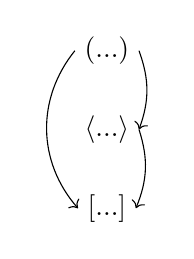
\begin{tikzpicture}
        \node (A) at (0,2) {\( (...) \)};
        \node (B) at (0,1) {\( \la ... \ra \)};
        \node (C) at (0,0) {\( [...] \)};

        \draw[->, bend left=20] (A.east) to node[right] {$\qU$} (B.east);
        \draw[->, bend left=20] (B.east) to node[right] {$\qD$} (C.east);
        \draw[->, bend right=40] (A.west) to node[left] {$\sw$} (C.west);
    \end{tikzpicture}
\end{center}

This shows that the proposed rewrite is indeed impossible.
\end{proof}

- Conclude that proofs are dinatural as they are compositions of naturals and dinaturals with no cycles
\newpage
\section{Some Big Result...}
\begin{theorem}
    Cor blimey look at the state of this stonking result!
\end{theorem}

\begin{proof}
    Bodge together all of the lemmas from the previous chapters and there you go.
    Easy.
    No bother at all.
\end{proof}

\newpage
\section{Conclusion}

\newpage
\bibliographystyle{plain}
\bibliography{references}

\end{document}